\subsubsection{Experiment 2}
\begin{figure}[htbp]
	\centering
    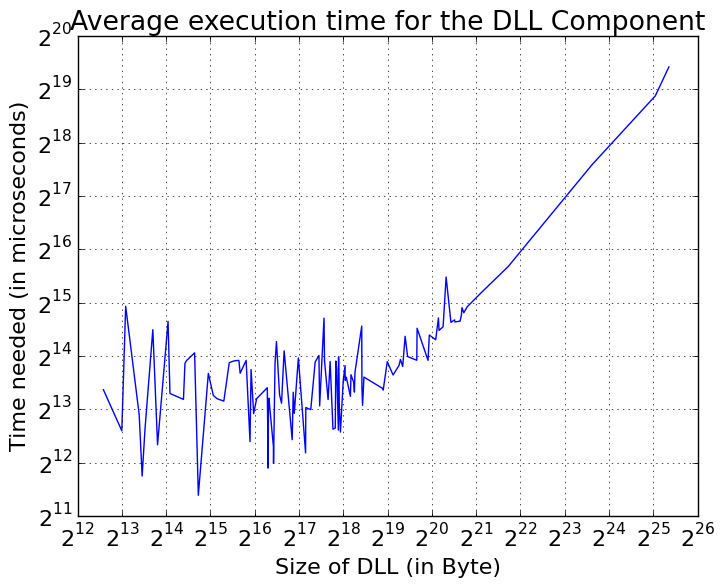
\includegraphics[width=\textwidth,height=0.45\textheight,keepaspectratio]{Evaluation/experiment2/result.png}
    \caption{Average execution time for sha256 file hashing}
    \label{fig:ex2_result}
\end{figure}
In Experiment 2 the performance impact of the \emph{\gls{DLL}} component is evaluated. Experiment 2 uses the same hardware and software setup as Experiment 1. As the result of Experiment 1 showed, that running the \emph{\gls{DLL}} component slowed down the execution of \emph{Google Chrome}, Experiment 2 tries to find the actual reason for that result. Looking at the code, and running time measurements on it leads to the sha256 file hashing slowing down the execution. Figure \ref{fig:ex2_result} shows the average of ten independent measurements. For file sizes between four kilobyte ($2^{12}$ byte) and one megabyte ($2^{20}$ byte), the needed time is roughly constant around 16 milliseconds ($2^{14}$ microseconds). Increasing the file size further than one megabyte results into increase of time for hashing the file. The graph uses logarithmic scaling with base two one both axis, which gives a better comparability of the actual result. Starting at one megabyte, doubling the file size will double the necessary time to create the sha256 hash. Most \glspl{DLL} are rather small (less than one megabyte) and will require constant time for file hashing. However, in contrast to that, some are very large (around 50 megabyte or even larger) and will require exponentially more time. An example for that can be found in \emph{Google Chrome's} used \glspl{DLL}. \emph{Chrome\_child.dll} with 40 megabyte and \emph{chrome.dll} with 30 megabyte make up most of the time that is spent for hashing during \emph{Chrome} process creation. As the initial callback function \syscall{PsSetLoadImageNotifyRoutine} is acting synchronous, so is the hashing of files. Therefore, the process is suspended for the whole time that is needed for hashing all \glspl{DLL}. A single process creation is delayed by the sum of the required time for hashing all \glspl{DLL}, which makes up a total of 2905253 microseconds, or 2.9 seconds. This performance decrease will always be existing when using a software that is creating file hashes, but it can be significantly improved by using a caching system or faster hashing algorithm.